\documentclass[./main.tex]{subfiles}
\graphicspath{{\subfix{./Abbildungen/}}}

\begin{document}
\renewcommand{\tasktitle}{Titel$^1$}
\renewcommand{\taskpoints}{3.5} %Gesamtpunktzahl der Aufgabe
\renewcommand{\taskweight}{17}
\aufgabenanfang % Beginn der Aufgabe
\footnotetext[1]{Test}

Dies ist ein Template zur Erstellung und Formatierung von IChO-Aufgaben (Klausurrunden 2–4) und Cds-Aufgaben in \LaTeX. 
Dies ist ein Beispiel für einen Einleitungstext zu einer Aufgabe. Es gibt zudem die Option diesen Text in einen Kasten zu setzen wie es ja bei der internationalen Runde üblich ist.\\
\textit{Für kursive Hervorhebung kann dies genutzt werden}. \textbf{Für fette Hervorhebung dies}.

\teilaufgabe{In diesem Bereich steht eine Teilaufgabe}{Hier kann ein Hinweis hinzugefügt werden}
\kasten{2.5cm}{
    Hiermit lässt sich ein Kasten erstellen zur Bearbeitung der Aufgabe.
    Die Länge des Kastens wird im Ersten Argument angegeben.
    Lösungskästchen folgen jeweils direkt auf die Aufgabenstellung – es gibt seit einigen Jahren keine Antwortbögen mehr!
    Musterlösung bzw Bewertungshinweise werden mit dem Command \textbackslash kommentar \{Hier direkt notiert\}:\\ %Zeilenumbruch
    \kommentar{Dies ist eine Musterlösung}\punkte{1}
}{Nur dieser Text erscheint in der Sch\"ulerversion}

Die folgenden Abschnitte enthalten einige Beispiel-Teilaufgaben. Die Aufgabenteile b) und c) dienen als Beispiele für Multiple-Choice-Aufgaben. 
\teilaufgabe{\operator{Kreuze an} welche Antwortm\"oglichkeiten hier richtig sind.}{Die Reihenfolge der richtigen Antworten wir in dem \textbackslash MC Command im 6.ten Argument mit einer Zeichenkette bspw.: oxoox, ausgedrückt die für die richtigen Antworten je ein x notiert}
Vor dem MC command folgt mit \textbackslash punkte wieder die Punktzahl\punkte{2}\par
\MC{A}{B}{C}{D}{E}{oxoox}
Bevorzugt wird eine richtig/falsch Auswahl, da hier ein falsch Ankreuzen auch bepunktet werden kann.\par % falls vor einem MC-Kasten noch Text stehen soll, muss an diesen ein \par angefügt werden!
\MCrf{A}{B}{C}{D}{E}{oxoox}
\teilaufgabe{\operator{Kreuze an} welche Antwortm\"oglichekeiten hier richtig sind.\punkte{1}}{}
\MCvAnfang
\MCv{x}{Eine richtige Lösung}
\MCv{o}{Eine falsche Lösung}
\MCv{o}{Eine falsche Lösung}
\MCv{o}{Eine falsche Lösung}
\MCv{o}{Eine falsche Lösung}
\MCv{o}{Eine falsche Lösung}
\MCvEnde 
Auch hier mit richtig/falsch möglich:\par
\MCvrfAnfang
\MCv{x}{Eine richtige Lösung}
\MCv{o}{Eine falsche Lösung}
\MCv{o}{Eine falsche Lösung}
\MCv{o}{Eine falsche Lösung}
\MCv{o}{Eine falsche Lösung}
\MCv{o}{Eine falsche Lösung}
\MCvrfEnde


Alternativ kann auch sortiert werden (zum Beispiel auch Moleküle nach ihrer Reaktivität):
\teilaufgabe{\operator{Sortiere} die Zahlen nach Größe.}{Dabei ist 5 die größte und 1 die kleinste Zahl.\punkte{2}}
\MSort{0}{29}{78}{-12}{103}{23415}







Aus ChemDraw lässt sich eine .eps Datei exportieren und hier wie ein Bild Einfügen.
Mit \ocscale kann die Größe aller Abbildungen gleich skaliert werden, wenn sie im Chemdraw auch gleich groß sind:
\renewcommand{\ocscale}{0.95}
\begin{scheme}[H]
    \centering
    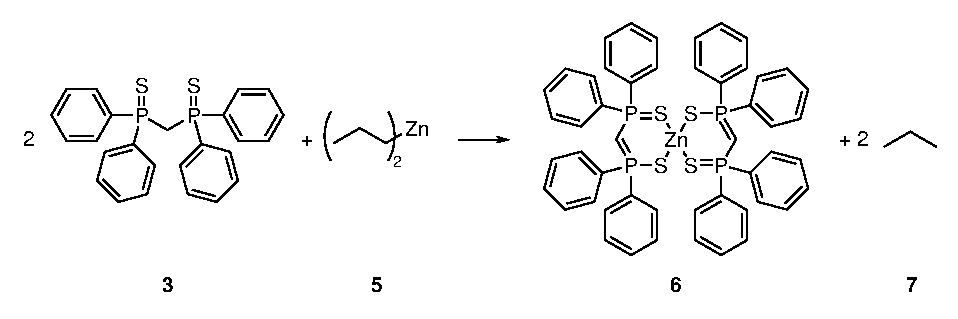
\includegraphics[scale=\ocscale]{Komplex.eps}
    \caption{Eine Synthese f\"ur die Tonne}
    \label{ACFKomplex}
\end{scheme}
Alternativ geht auch die Feststellung der Breite mit linewidth:
\begin{scheme}[H]
    \centering
    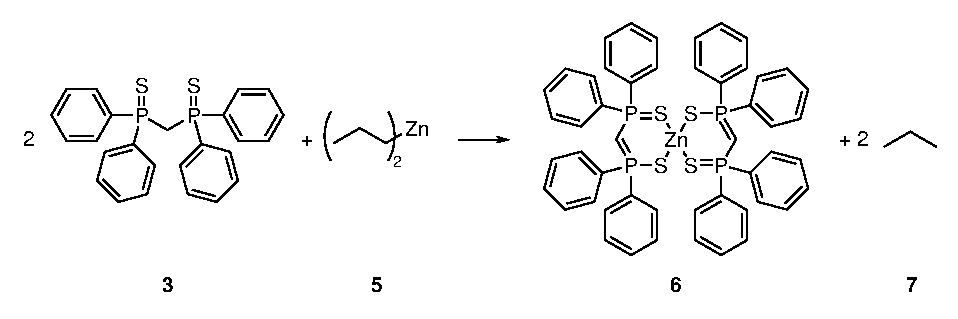
\includegraphics[width=0.85\linewidth]{Komplex.eps}
    \caption{Zweite Synthese f\"ur die Tonne}
\end{scheme}

Zu der Darstellung der OC- Lösungskästchen dient der Befehl:\\
In der folgenden Teilaufgabe folgt das Einfügen von OC Formeln Bildern und OC Kästchen. 

\ocanfang
\oc{\textbf{1}}{
\includegraphics[scale=\ocscale]{beta_lacton.eps}}{}
\oc{\textbf{2}}{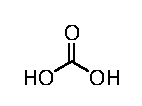
\includegraphics[scale=\ocscale]{H2CO3.eps}}{}
\oc{\textbf{3}}{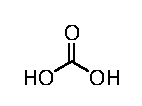
\includegraphics[width=0.5\linewidth]{H2CO3.eps}}{}
\ockasten{112}{4}
\ocende
% \kastenarray
%     [] % Breite (kann weggelassen werden, dann an Inhalt angepasst)
%     {4cm} % Höhe
%     [0cm] % Abstand zwischen den Kästchen (kann weggelassen werden, dann 0cm)
%     [f] %t oder f: t - kein Abstand unter Kasten; f - Abstand unter Kasten (Optional; wenn weggelassen dann =t)
%     {Q,W} % Bezeichnungen
%     {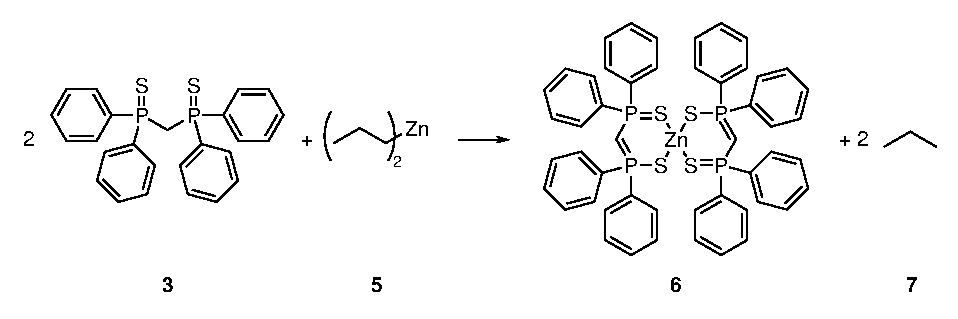
\includegraphics[width=5.5cm]{Komplex.eps},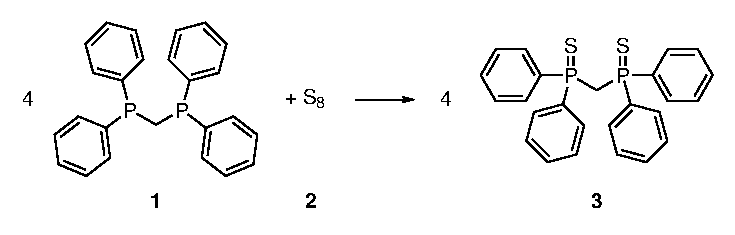
\includegraphics[width=5.5cm]{Ligand.eps}}% Inhalte mit Kommata seperieren
Man kann diese auch aneinander Reihen:
Noch zwei Kastenarrays.
% \kastenarray[7cm]{7cm}{1,2}{Molekuel1,Molekuel2}

\kasten{16cm}{
Reaktion erster Ordnung: \ch{A -> B}\punkte{1}
\begin{align*}
    v(t)&=-\dd{[\ch{A}]}{t}=k\cdot[\ch{A}]\punkte{1}\\
    a(t)&=-\dd[2]{[\ch{A}]}{t}\quad\kommentar{Auch höhere Ableitungen sind möglich.}\\
    \intertext{Mit \textbackslash intertext kann man auch Text in Gleichungen einfügen.}\\
    \frac{\textnormal{d}[\ch{A}]}{[\ch{A}]}&=-k\,\textnormal{d}t\\
    \int_{[\ch{A}]_0}^{[\ch{A}]}\left(\frac{1}{[\ch{A}]}\right)\,\textnormal{d}[\ch{A}]&=\int_0^t -k\,\textnormal{d}t\punkte{1}\\
    &=\ln[\ch{A}]-\ln[\ch{A}]_0=\ln\left(\frac{[\ch{A}]}{[\ch{A}]_0}\right)\\
    \Rightarrow [\ch{A}]&=[\ch{A}]_0\cdot\exp{-k\cdot t}\punkte{1}
\end{align*}
\kommentar{1P für Rkt. 1. Ordnung, 1P für Geschwindigkeitsgesetz, 1P für Integrieren, 1P für richtiges Ergebnis}
}{}
\newpage
\teilaufgabe{\operator{Male} das Mandala aus.\punkte{69}}{Dies wurde nur hinzugefügt, um \textbackslash punkteausgabe zu zeigen.}
\begin{scheme}[H]
    
\includegraphics[width=\linewidth]{mandala.jpg}
\end{scheme}
\punkteausgabe

Hier wurde Punkteausgabe benutzt, da die Aufgabe keine Form benutzt, die die Punkte bereits selbst ausgibt.

\teilaufgabe{\operator{Einige Leute} wollen den SuS bereits einen Text in den Antwortkasten schreiben.}{Um dies flexibel zu ermöglichen, kann man \textbackslash selfkasten nutzen.}
\selfkasten{5cm}{
    \sol{Test}\punkte{1}\\
    Hallo das ist ein Paragraphlol
}

Formeln im Text können mit align und labeln erstellt werden, um verlinkt zu werden z.B. Gleichung \ref{G:test-Gl}:
\begin{align}
    pV &= nRT \label{G:test-Gl}\\
    a &= b
\end{align}
\begin{equation*}
    Q = I \cdot t
\end{equation*}
In Gleichung ist das ideale Gasgesetz gezeigt\ldots 
Im Text sollten Vorzeichen wie bei $\delta-$/$\delta+$ besser au\ss{}erhalb des Mathemodusses stehen, aber ein richtiges Minuszeichen verwenden: $\delta$+/$\delta$\textminus{}\\
Auch innerhalb eines Kastens sind solche Formelumgebungen möglich. Zudem sind Punkte und Kommentare in aligns möglich:\\
\kasten{5cm}{
\begin{align*}
    y = x^2 \punkte{2}\kommentar{\ Kommentar}
\end{align*}
Dies ist die Antwort. Dies ist Antwortsatz 2.
}{}
Hier kommt mal eine andere Aufz\"ahlung:\\
\begin{enumerate}[(i)]
    \item Hallo
    \item Tschüss
\end{enumerate}

Ein bisschen Millimeterpapier:\\
\kasten{10cm}{
\begin{center}
    \millipapier{1}{16}{9}
\end{center}
}{}


Zwei Tabellen voller Daten:
\begin{table}[H]
    \caption{Tabelle mit verschiedenen thermodynamischen Daten ausgew\"ahlter Stoffe bei $\SI{298}{\kelvin}$.}
    \label{tab: 2025-10-3_therm. Daten}
    \centering
    \begin{tabular}{|c|C{1.5cm}|C{1.5cm}|C{1.5cm}|C{1.5cm}|}
    \hline
        & \ch{CH4} & \ch{H2O} & \ch{CO} & \ch{H2}\\\hline
        $\Delta_fH^{\circ}_m$ / $\si{\kilo\joule\per\mole}$ & -74,85 & -241,8 & -110,5 & 0\\\hline
        $S^{\circ}_m$ / $\si{\joule\per\mole\per\kelvin}$ & 186,2 & 188,9 & 198,0 & 130,6\\\hline
        $C_{p, m}$ / $\si{\joule\per\mole\per\kelvin}$ & 35,31 & 33,58 & 29,14 & 28,82\\\hline
    \end{tabular}
\end{table}

\begin{table}[H]
    \caption{Tabelle mit verschiedenen thermodynamischen Daten ausgew\"ahlter Stoffe bei $\SI{298}{\kelvin}$.}
    \label{tab: 2025-10-3_therm. Daten2}
    \centering
    \begin{tabular}{cC{1.5cm}C{1.5cm}C{1.5cm}C{1.5cm}}
    \toprule
        & \ch{CH4} & \ch{H2O} & \ch{CO} & \ch{H2}\\\midrule
        $\Delta_fH^{\circ}_m$ / $\si{\kilo\joule\per\mole}$ & -74,85 & -241,8 & -110,5 & 0\\
        $S^{\circ}_m$ / $\si{\joule\per\mole\per\kelvin}$ & 186,2 & 188,9 & 198,0 & 130,6\\
        $C_{p, m}$ / $\si{\joule\per\mole\per\kelvin}$ & 35,31 & 33,58 & 29,14 & 28,82\\\bottomrule
    \end{tabular}
\end{table}

\aufgabenende
\end{document}
